\begin{frame}[t,label=case-t1-004]{T1 Visibility / 004}{Flat trace 不能确定一个很长的 T1}
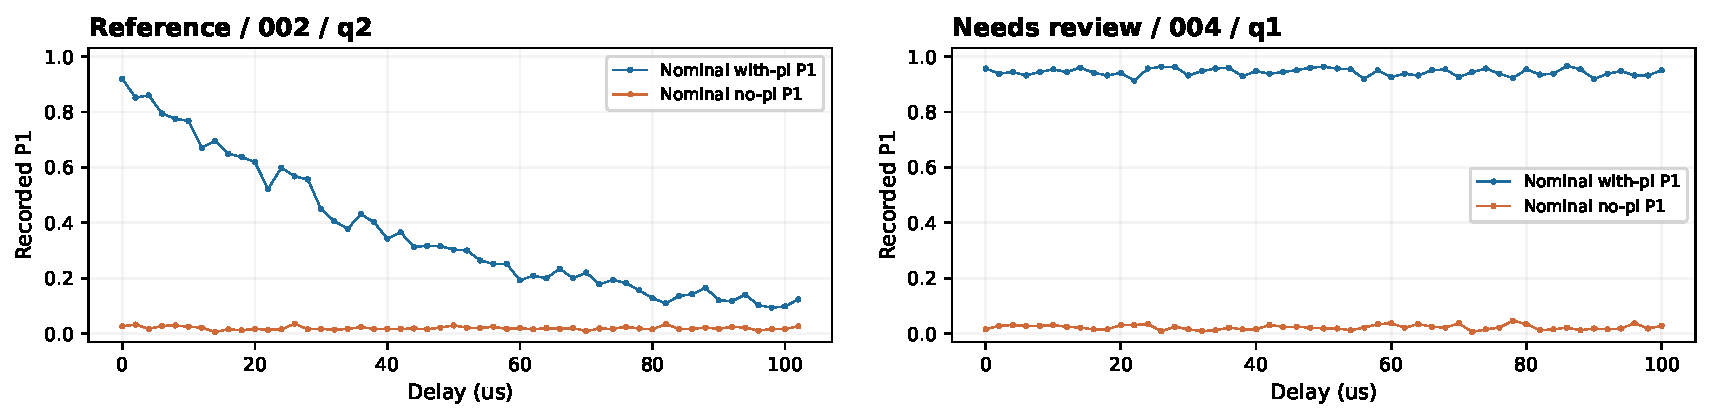
\includegraphics[width=\linewidth]{figures/t1-004.pdf}
\vspace{-1.5mm}
{\fontsize{8.4}{10}\selectfont\color{Muted} Contrast fit: $R^2=0.008$; lifetime reaches $10000\,\mu s$ fit bound; lifetime unresolved\par}
\vspace{1mm}{\fontsize{8.7}{10.4}\selectfont\renewcommand{\arraystretch}{1.08}\begin{tabularx}{\linewidth}{@{}>{\bfseries\color{Navy}}p{1.35cm}X@{}}
观察 & Nominal with-pi P1：0.956 $\to$ 0.950（0--100 us）；几乎没有 resolved decay。 \\
可能原因 & Lifetime 超出窗口；delay 未实际改变；readout 前重激发；channel 或 acquisition 有误。 \\
验证 & 核对 executed sequence 与 time units；重复 preparation reference，再扩大 delay window。
\end{tabularx}}
\vfill
{\fontsize{6.5}{8}\selectfont\color{Muted} Source: 0918 / T1 Visibility / 002, 004; raw CSV replotted. P1 channel preparation order inferred; metrics fit contrast.\par}
\end{frame}

\begin{frame}[t,label=case-readout-008]{GMM Readout Clusters / 008}{Preparation label 不等于可可靠区分的 state}
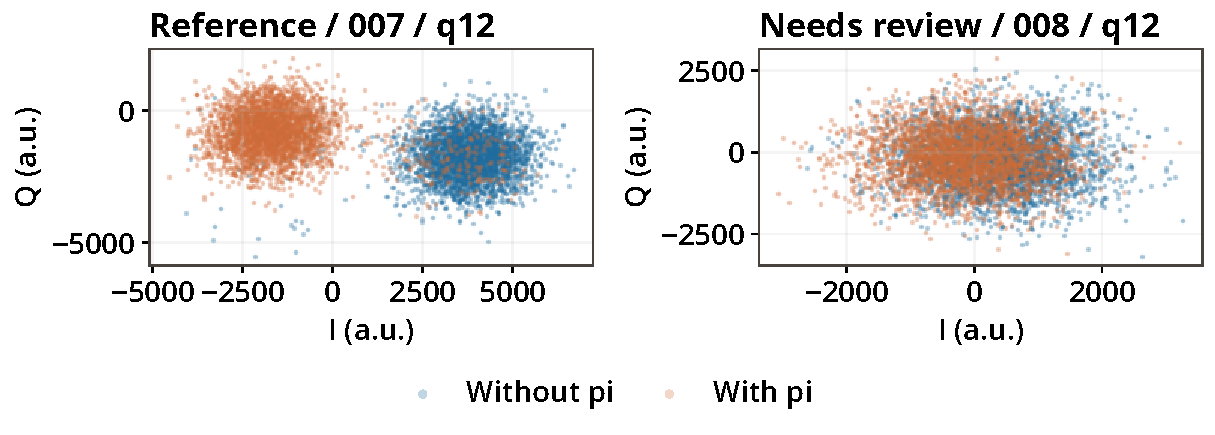
\includegraphics[width=\linewidth]{figures/readout-008.pdf}
\vspace{-1.5mm}
{\fontsize{8.4}{10}\selectfont\color{Muted} Held-out linear classifier: balanced accuracy $61.70\%$; not original GMM fidelity\par}
\vspace{1mm}{\fontsize{8.7}{10.4}\selectfont\renewcommand{\arraystretch}{1.08}\begin{tabularx}{\linewidth}{@{}>{\bfseries\color{Navy}}p{1.35cm}X@{}}
观察 & Held-out linear balanced accuracy = 61.70\%；nominal preparation groups 重叠。 \\
可能原因 & Preparation pulse 不准；probe setting 不合适；measurement 期间 relaxation；measurement chain noise。 \\
验证 & 先验证 preparation / Rabi，再检查 probe frequency、integration window 和 demodulated time trace。
\end{tabularx}}
\vfill
{\fontsize{6.5}{8}\selectfont\color{Muted} Source: 0918 / GMM Readout Clusters / 007, 008; raw CSV replotted. Classifier predicts preparation labels; not isolated readout error.\par}
\end{frame}

\begin{frame}[t,label=case-rabi-003]{Rabi Oscillation / 003}{Noise-like trace 中，fitter 仍然会返回 period}
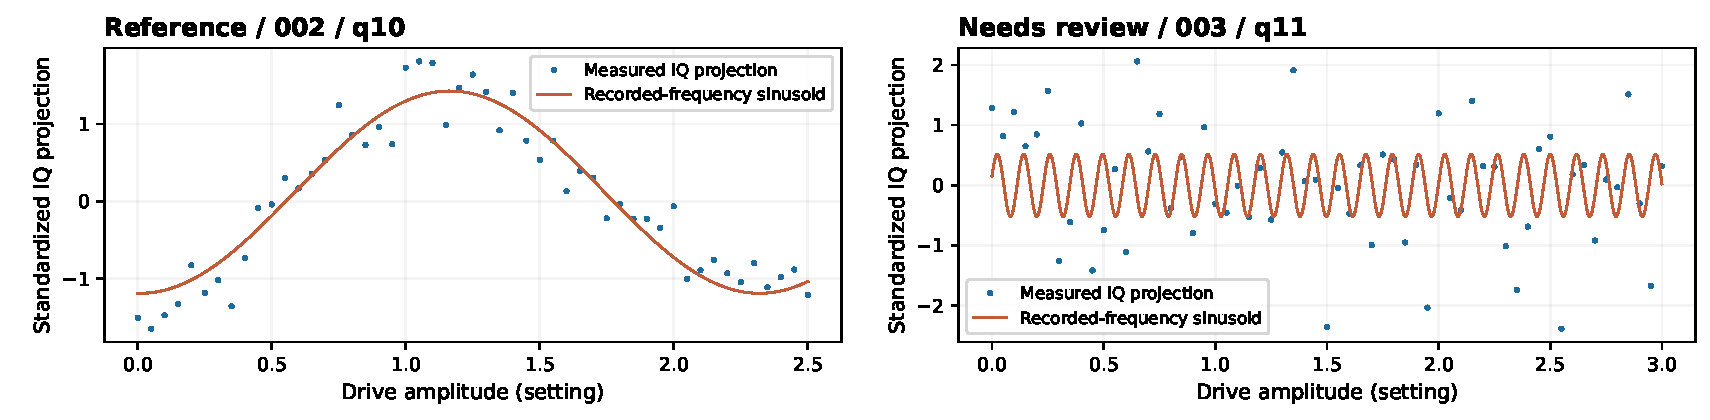
\includegraphics[width=\linewidth]{figures/rabi-003.pdf}
\vspace{-1.5mm}
{\fontsize{8.4}{10}\selectfont\color{Muted} IQ-projection fit: $R^2=0.130$; coverage $25.44$ cycles; $2.4$ samples/cycle\par}
\vspace{1mm}{\fontsize{8.7}{10.4}\selectfont\renewcommand{\arraystretch}{1.08}\begin{tabularx}{\linewidth}{@{}>{\bfseries\color{Navy}}p{1.35cm}X@{}}
观察 & 没有清晰完整 cycle；R2=0.130；每个 fitted cycle 仅 2.36 个 samples。 \\
可能原因 & Drive / readout contrast 不足、frequency 不准或 pulse path 问题；candidate 高频也可能是 noise fitting。 \\
验证 & 先验证 spectroscopy 与 readout，再重复 sweep；不能直接采用 fitted half-period 作为 pi amplitude。
\end{tabularx}}
\vfill
{\fontsize{6.5}{8}\selectfont\color{Muted} Source: 0918 / Rabi Oscillation / 002, 003; raw CSV replotted. IQ projection is standardized independently; its sign is arbitrary.\par}
\end{frame}

\begin{frame}[t,label=case-rabi-007]{Rabi Oscillation / 007}{高 fit score 不保证 period 已被测到}
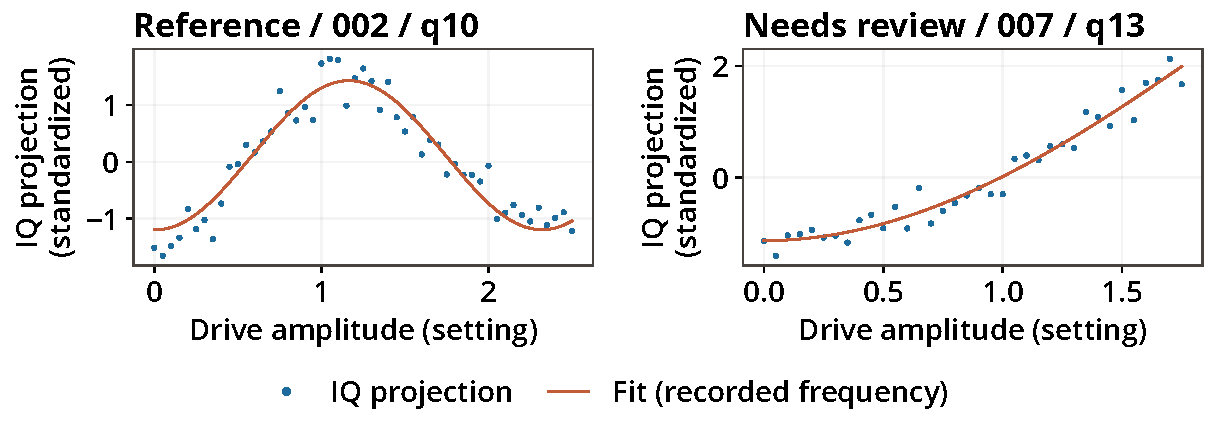
\includegraphics[width=\linewidth]{figures/rabi-007.pdf}
\vspace{-1.5mm}
{\fontsize{8.4}{10}\selectfont\color{Muted} IQ-projection fit: $R^2=0.959$; coverage $0.22$ cycles; $159.7$ samples/cycle\par}
\vspace{1mm}{\fontsize{8.7}{10.4}\selectfont\renewcommand{\arraystretch}{1.08}\begin{tabularx}{\linewidth}{@{}>{\bfseries\color{Navy}}p{1.35cm}X@{}}
观察 & Scan 仅覆盖 candidate cycle 的 0.22；period 很大部分来自 extrapolation。 \\
可能原因 & Amplitude window 太短；局部 response 被误当作完整 sinusoid；模型可辨识性不足。 \\
验证 & 在合适的控制范围内扩大 amplitude scan；观察 turning point 与 return；验证 pi endpoint。
\end{tabularx}}
\vfill
{\fontsize{6.5}{8}\selectfont\color{Muted} Source: 0918 / Rabi Oscillation / 002, 007; raw CSV replotted. IQ projection is standardized independently; its sign is arbitrary.\par}
\end{frame}

\begin{frame}[t,label=case-spectroscopy-008]{Qubit Spectroscopy / 008}{Scan boundary 限制了 resonance center 的判断}
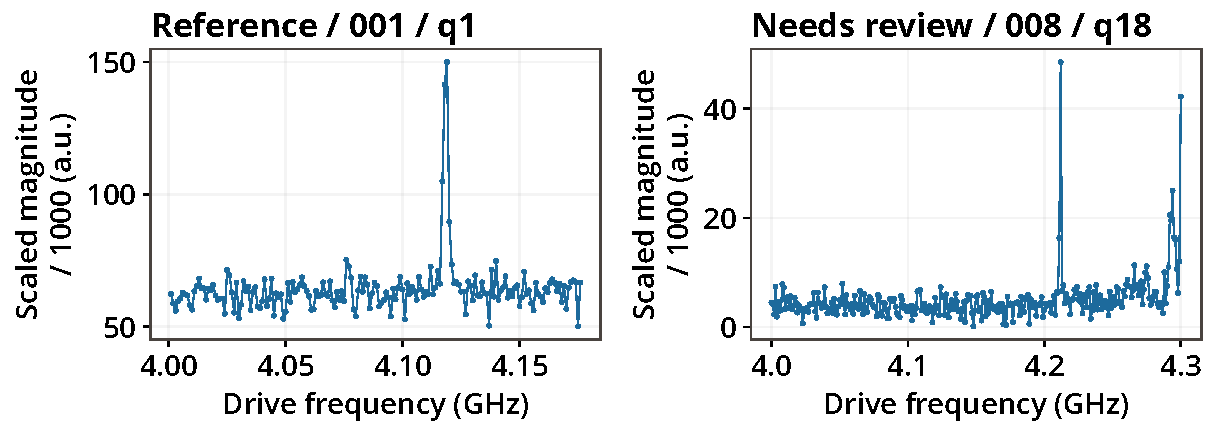
\includegraphics[width=\linewidth]{figures/spectroscopy-008.pdf}
\vspace{-1.5mm}
{\fontsize{8.4}{10}\selectfont\color{Muted} IQ single-line diagnostic: $R^2=0.312$; step $1.00$ MHz; FWHM $13.30$ MHz\par}
\vspace{1mm}{\fontsize{8.7}{10.4}\selectfont\renewcommand{\arraystretch}{1.08}\begin{tabularx}{\linewidth}{@{}>{\bfseries\color{Navy}}p{1.35cm}X@{}}
观察 & Candidate center=4.300 GHz 位于 scan 边界；不能完整观察两侧 response。 \\
可能原因 & Feature 延伸到窗口外、多个 transitions 或 baseline 变化；边界值不是已测定的 center。 \\
验证 & 扩大 frequency window 观察两侧；检查 candidate feature 的复现性与 drive-strength dependence。
\end{tabularx}}
\vfill
{\fontsize{6.5}{8}\selectfont\color{Muted} Source: 0918 / Qubit Spectroscopy / 001, 008; raw CSV replotted. Magnitude plotted; reported R2 and FWHM are from IQ-projection diagnostic.\par}
\end{frame}

\begin{frame}[t,label=case-spectroscopy-005]{Qubit Spectroscopy / 005}{Fit score 不能补足 frequency resolution}
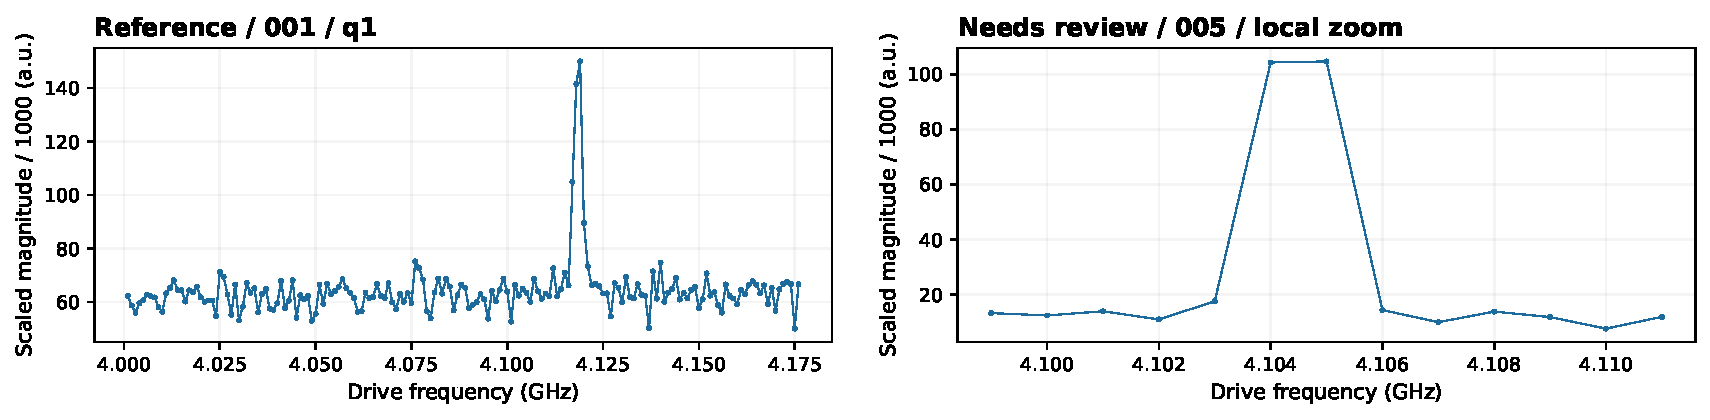
\includegraphics[width=\linewidth]{figures/spectroscopy-005.pdf}
\vspace{-1.5mm}
{\fontsize{8.4}{10}\selectfont\color{Muted} IQ single-line diagnostic: $R^2=0.965$; step $1.00$ MHz; FWHM $0.50$ MHz\par}
\vspace{1mm}{\fontsize{8.7}{10.4}\selectfont\renewcommand{\arraystretch}{1.08}\begin{tabularx}{\linewidth}{@{}>{\bfseries\color{Navy}}p{1.35cm}X@{}}
观察 & Frequency step=1.00 MHz，candidate FWHM=0.50 MHz；采样不足。 \\
可能原因 & 实际窄 resonance 或 isolated outlier；现有 grid 无法可靠区分，也不支持过高 linewidth precision。 \\
验证 & 在 feature 附近使用更小 frequency step，并重复采样；比较 peak / dip 的宽度与 reproducibility。
\end{tabularx}}
\vfill
{\fontsize{6.5}{8}\selectfont\color{Muted} Source: 0918 / Qubit Spectroscopy / 001, 005; raw CSV replotted. Magnitude plotted; reported R2 and FWHM are from IQ-projection diagnostic.\par}
\end{frame}

\begin{frame}[t,label=case-ramsey-008]{T2 Ramsey / 008}{Envelope 结构超出单一 exponential model}
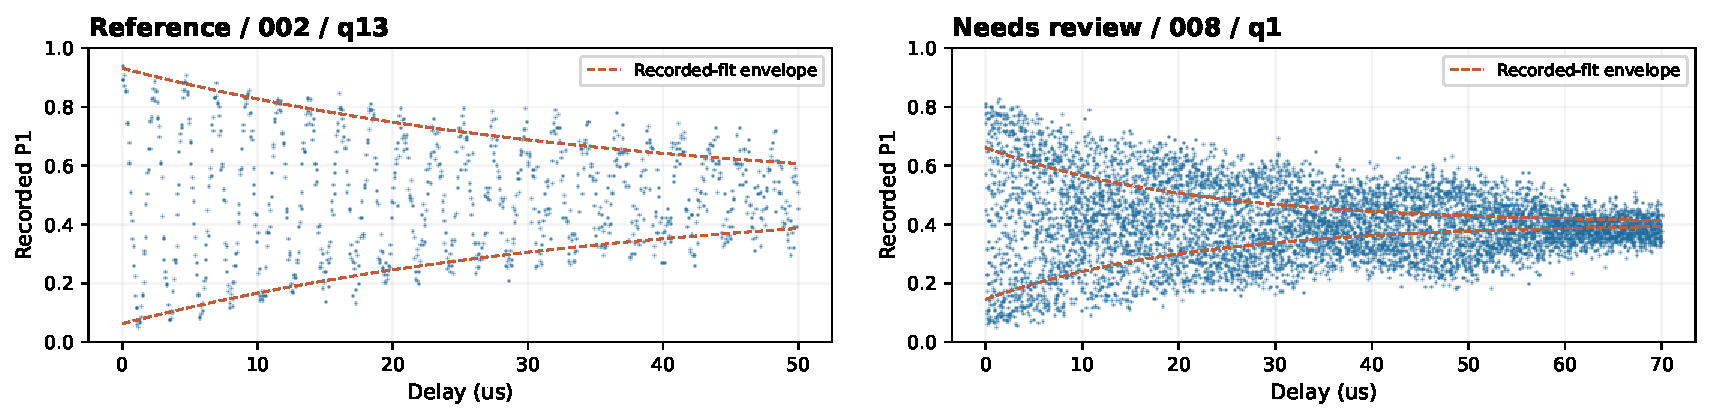
\includegraphics[width=\linewidth]{figures/ramsey-008.pdf}
\vspace{-1.5mm}
{\fontsize{8.4}{10}\selectfont\color{Muted} Recorded Ramsey fit: $R^2=0.328$; candidate $T_2^*=21.78\,\mu s$; residual correlation $0.38$\par}
\vspace{1mm}{\fontsize{8.7}{10.4}\selectfont\renewcommand{\arraystretch}{1.08}\begin{tabularx}{\linewidth}{@{}>{\bfseries\color{Navy}}p{1.35cm}X@{}}
观察 & Dense oscillation trace 在约 40--50 us 重新变宽；single-envelope fit 不能覆盖全部结构。 \\
可能原因 & Multiple frequencies / beating、drift 或 readout / noise 变化；不能仅凭图确认 low-frequency noise。 \\
验证 & 检查 cycle-resolved trace 与 residual；重复 acquisition；比较 fit window、envelope 与 echo。
\end{tabularx}}
\vfill
{\fontsize{6.5}{8}\selectfont\color{Muted} Source: 0918 / T2 Ramsey / 002, 008; raw CSV replotted. Reference also flagged; envelope shown, not the full fitted oscillation.\par}
\end{frame}

\begin{frame}[t,label=case-resonator-006]{Resonator Spectroscopy / 006}{First-point spike 是 resonance 还是 acquisition transient？}
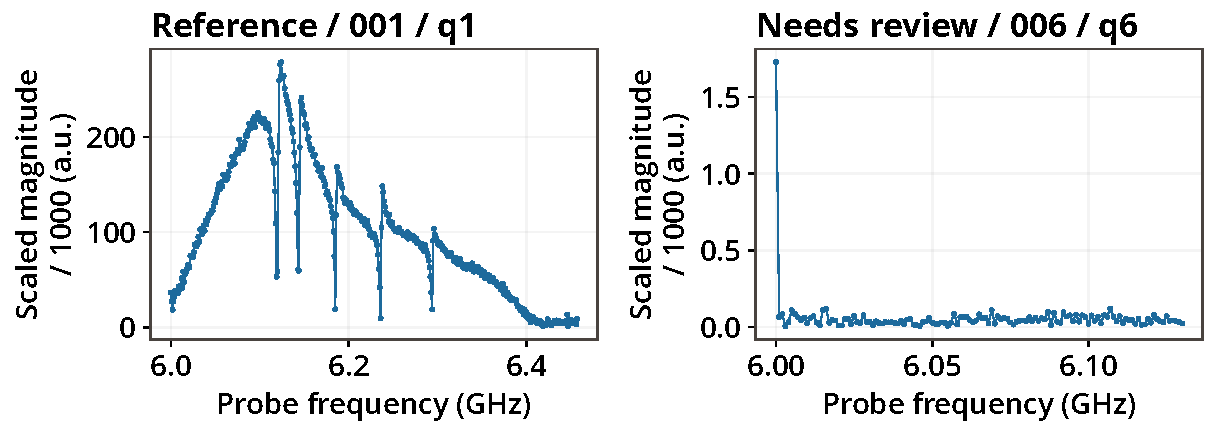
\includegraphics[width=\linewidth]{figures/resonator-006.pdf}
\vspace{-1.5mm}
{\fontsize{8.4}{10}\selectfont\color{Muted} Descriptive screen only: window 6.000--6.130 GHz; no validated transfer-function fit\par}
\vspace{1mm}{\fontsize{8.7}{10.4}\selectfont\renewcommand{\arraystretch}{1.08}\begin{tabularx}{\linewidth}{@{}>{\bfseries\color{Navy}}p{1.35cm}X@{}}
观察 & Scaled magnitude 首点约 1728，次点约 66，后续 median 约 41；窗口内无 resolved interior resonance。 \\
可能原因 & Settling / acquisition discontinuity、edge / out-of-window resonance，或 useful signal 不足。 \\
验证 & 加入 settling 后重测首点；反向 sweep；扩大窗口并同时检查 phase / IQ。
\end{tabularx}}
\vfill
{\fontsize{6.5}{8}\selectfont\color{Muted} Source: 0918 / Resonator Spectroscopy / 001, 006; raw CSV replotted. Independent scales/settings; multiple features can be normal.\par}
\end{frame}
